\chapter{Platformalapú rendszertervezési és -szimulációs módszertan}
Ebben a fejezetben kerülnek bemutatásra a téma kapcsán létrejött saját eredmények. Először a megoldás lehetséges módjai kerülnek bemutatásra az előnyeikkel és hátrányaikkal együtt.
A második alfejezet a rendszerek SysML v2-ben történő modellezéséhez létrehozott módszertant mutatja be, amelybe beleépülnek a szimulációs technológiákhoz létrehozott módszerek.
Végül egy konkrét esettanulmányon keresztül bemutatásra kerülnek a leírt módszerek.

\section{Lehetséges megközelítések}
A modellalapú rendszertervezési és a szimulációs technológiák integrálása módosításokat követel mind a két oldal modelljeiben.
Ezek a módosítások és tervezési módszerek a két terület közötti kapcsolat, egy kölcsönös megfeleltetés miatt elengedhetetlenek.
Azonban több különböző lehetőségünk van, ennek a megvalósítására.
Ez az alfejezet ezeket a megközelítéseket veszi sorra és hasonlítja össze.

    \subsection{Szimulációs fogalmak bevezetése a rendszermodellbe}
    A rendszermodell tekintetében a leglátványosabbak ezek a változások, mivel itt ténylegesen meg kell jelenni a másik szakterületnek, hogy az beolvadhasson a fejlesztési folyamatba.
    A szimulációs fogalmak bevezetésére két módszert dolgoztunk ki, amelyeket részletesen tárgyalunk majd.

        \subsubsection{Annotáció alapú leképezés}
        Az új fogalmak és tulajdonságok bevezetésére a legkézenfekvőbb megoldás a SysML v2 nyújtotta lehetőség különböző metaadatok bevezetésére.
        A megoldás lényege, hogy létrehozunk egy importálható fájlt amely minden fontos fogalomhoz tartalmaz egy-egy annotációt, amivel az adott eleme bevezethető. Gyakorlatilag kézzel megcímkézzük, hogy melyek a fizikai és logikai elemek, melyik kapcsolat milyen típusú, stb.
        
        Ezen kívül lehetőség van szabályokat megadni, amelyek segítenek megakadályozni a hibás használatot, például nem jelölhetjük külön szimulációs egységnek (Például FMU-k.) a követelményeket vagy a köztük lévő logikai kapcsolatot.
        
        Ezzel a megoldással, a fogalmak bevezetése abból áll, hogy minden elemet ellátunk a megfelelő annotációval és ezek alapján a leképezést létrehozó vagy felhasználó programok ezek segítségével tudják értelmezni, bejárni a rendszermodellt szimulációs szemszögből nézve.

        \subsubsection{Szimulációs modellvetület bevezetése}
        A másik lehetőség, ha bevezetünk egy konkrét területet a modellben --~egyfajta nézetet~-- amely leírja a szimulációs modellt.
        A rendszermodellezésben alapvetően jelen van ez a szemlélet, a rendszerek tervezésénél egy logikai és egy fizikai modellel dolgoznak a rendszermérnökök.
        
        Ennél a megközelítésnél egy ezekhez hasonló, harmadik vetületet hozunk be a rendszermodellbe és a rendszermodell elemeit explicite összekötjük az azokat reprezentáló szimulációs elemek modelljével.
        Ezzel a megoldással a szimulációkhoz kapcsolódó fogalmak, csak a vonatkozó nézetben jelennek meg.
        
        Magának a nézetnek a megvalósításához célszerű készíteni egy nyelvi kiterjesztést.
        Ez a SysML v2 adta lehetőség arra, hogy szakterület specifikus típusokat hozhassunk létre.
        Ennek az eszköznek a használata célszerűbb ennél a megközelítésnél, mert itt egy konkrét szakterület szerinti modellt alkotunk.
        Nincs szükség az annotációk flexibilitására, cserébe a használata egyszerűbb, jobban kikényszeríthető a megfelelő struktúra alkalmazása, mint ha csak különböző annotációkat adnánk az egyes elemekhez.

        \subsubsection{Lehetőségek összehasonlítása} \label{sec:ReMoOsszehasonlitas}
        Az annotáció alapú megközelítés előnye könnyen látható. Az, hogy a meglévő modell elemeit felcímkézzük, lehetővé téve a leképezést, azt jelenti, hogy minimális többletmunkára van szükség az eddigiekhez képest.
        A kevesebb nézet szerinti modellezés kevesebb munkát igényel, így a fejlesztés gyorsabban haladhat.

        Továbbá mivel az annotációk bármilyen modellre elhelyezhetőek, annak struktúrájától függetlenül, így a már meglévő modellek esetében is könnyű bevezetni a szimulációkat a további fejlesztések támogatására.
        Ez a szempont jelenleg még kevésbé jelentős, mivel magának a SysML v2-nek a bevezetése sem kezdődött még el.

        Ebből viszont az is következik, hogy más megközelítés használata esetén ez a legmegfelelőbb időpont, a szimulációk integrációjára is, mert jelenleg mindenképpen várható a modellek és módszertanok leváltása a SysML v2 szabvány megjelenése után.
        Egyszerűbb ha a többi komoly változás is megtörténik ezekkel együtt, mint utólag bevezetni új megközelítéseket amikor már végre újra normalizálódtak a fejlesztési folyamatok egy nagy váltás után.
        
        Az annotációkon alapuló módszernek azonban van négy komoly hátránya is, melyek a második módszer használata mellett nem okoznak problémát.

        Ha a teljes modellben jelen vannak az új szakterület fogalmai, az azt jelenti, hogy mindenkinek tisztában kell lenni azokkal, hogy dolgozni tudjon.
        Ez azt jelenti, hogy minden rendszermérnököt külön szimulációs technológiákra vonatkozó képzésben kell részesíteni.
        Ráadásul az extra képzésben részesített szakemberek nyilvánvalóan nem tudják olyan hatékonyan végezni ezt a munkát, mint azok, akik külön erre a területre specializálódtak.

        Az annotációs módszer második hátránya, hogy bármilyen modellstruktúrát megenged, nem kényszeríti ki egy jól kidolgozott módszertan követését.
        Egy általános modellstruktúra leképezéséhez a feladatot ellátó szoftvereknek is jóval komplexebbnek kell lenniük, mintha egy előre ismert struktúra mentén dolgoznának.

        A harmadik probléma, hogy az elemeken elhelyezett annotációk egyféle képpen címkézik fel a modellt, azaz egyetlen szimulációs modellt írnak le.
        A szimulációk során azonban rendszerint számos különböző modellt használnak, az aktuális igényeknek megfelelően, ezek között szükséges, hogy lehessen váltani, a komponensek különböző modelljeiből több összeállítást készíteni.
        
        Ehhez vegyünk például egy robotot és annak tápegységét.
        Amikor a tápegységet fejlesztjük, fontos, hogy a benne zajló jelenségeket minél pontosabban modellezzük. Például egy kapcsoló üzemű tápegységnél a benne használt félvezető alkatrészer pontos viselkedése elengedhetetlen a hatékonyság és a kimenő vezetékeken megjelenő zaj optimalizálásához, a követelmények teljesülésének vizsgálatához.
        Azonban amikor a robotunk vezérlését teszteljük, akkor rendszerint érdektelen számunkra, hogy tökéletesen pontosan ismerjük a fenti paramétereket, az a fontos, hogy az adott mozgások okozta terhelést képes-e kielégíteni a rendszer, illetve körülbelül mekkora a fogyasztása.
        Ezt a problémát úgy oldják meg, hogy több, különböző részletességű modellt készítenek, az egyes feladatokhoz.
        Persze használható minden feladatra a legrészletesebb modell, azonban az extra részletek sokszor nem jelentenek lényeges különbséget, míg a szimuláció számításigényét jelentősen megemelhetik.

        A szimulációs modellhez tartozó nézet bevezetése megoldja a fenti problémákat.
        Azzal, hogy egy konkrét modellrészletre korlátozzuk a speciális tudást igénylő munkafolyamatokat, lehetőség nyílik egyetlen, specializált szakemberekből álló csoportra bízni ezt a feladatot.
        A többi mérnöknek nem kell további képzés, a specializált szakemberek pedig jobb minőségű munkát végezhetnek a terület behatóbb ismeretének köszönhetően.

        Az előre ismert struktúra és a doménspecifikus modellezési eszközök bevezetése megkönnyíti a modelleket és az eszköztámogatást készítők munkáját is.

        Azzal, hogy a különböző szimulációs funkciókat nem kötjük hozzá direkt módon a rendszermodell elemeihez, lehetőség nyílik, hogy a szimulációs nézetben több szimulációs modellt is kapcsoljunk egy rendszerkomponenshez.
        Ez lehetővé teszi az eltérő részletességű modellek bevezetését, valamint a HiL és SiL technológiákhoz kapcsolódó szimulációs modellek is könnyen kezelhetőek egy-egy extra verzióként.

        Azonban legfontosabb különbség a két módszer között a fejlesztés nyomonkövethetősége. A szimulált rendszer egy virtuális reprezentációja a valósnak.
        A kritikus rendszereknél --~ahol a rendszertervezésnek kiemelt jelentősége van~--, mindennél fontosabb, hogy minden döntés, követelmény és felelősség nyomonkövethető legyen a teljes fejlesztési folyamatban.
        Azzal, hogy a rendszermodellt egyszerűen felcímkézzük a megfelelő jelölésekkel, elveszítjük az utolsó lépést az eddig gondosan épített nyomonkövethetőségből.
        Persze a konkrét elemekig ennek nyomán jutottunk el, így jelen van bizonyos mértékű nyomonkövethetőség, de ez messze nem tökéletes.
        Ez az alfejezet éppen arról szól, hogy a szimulációs modell kapcsán felmerülő legfontosabb tervezői döntéseket mérlegeljük, és éppen ezek azok, amelyeket annotációkkal nem tudunk nyomonkövetni, miközben a rendszertervezés legalapvetőbb szabálya, hogy minden lépés nyomonkövethető és indokolható kell legyen.
        Az új nézet bevezetésé mellett nem áll fent ez a probléma, a rendszer vetületeiben eddig is minden tény szépen nyomonkövethető volt a teljes modellen keresztül.

        A fentiek alapján látható, hogy az új nézet bevezetése jobban illeszkedik a technológiák alkalmazásához, jobb minőségű modelleket tesz lehetővé és a speciális szaktudás igényének csökkentésével az ilyen módszerek egyszerűbben és olcsóbban vezethetőek be a gyakorlatban.
        Ezek alapján a további munka során erre a megközelítésre összpontosítunk.

    \subsection{Szimulációs modell architektúrák}
    A szimulációs modellek esetében a változások azért szükségesek, hogy a rendszermodell megfelelően leképezhesse a szimulációs modelleket.
    Itt inkább tervezési konvenciókról, megkötésekről van szó, mivel egy teljesen szabadon készült modell leképezése jóval bonyolultabb feladat, mintha valamilyen előre ismert sémát használunk.

        \subsubsection{Leképezés a Modelica teljes eszközkészletével}
        A Modelica nyelvet kifejezetten fizikai rendszerek leírására és szimulációjára fejlesztették ki.
        Ennek köszönhető gazdag eszközkészlete van a különböző jelenségek leírására.
        
        Az első megközelítés, hogy ezeknek az eszközöknek mindegyikét szabadon használjuk a rendszer leírásához, mivel a minél pontosabb modellek érdekében hozták létre ezeket a nyelvi elemeket.
        Ilyen eszköz a külső változók használata, amelyek a környezeti hatások, mint például a gravitáció megadását teszik lehetővé. Ez azért hasznos, mert például égitestek modelljében, csak azt tüntetjük fel, hogy hat a testre ilyen erő és ez hogyan befolyásolja, azonban a számítását a környezetre bízza. Így könnyebben újrahasználható és logikusabban strukturált modelleket kapunk, hiszen nem egy adott égitesttől függ, hogy milyen erők hatnak rá hanem a környezetét alkotó égitestek alkotta rendszer sajátja ez a dinamika.
        
        A másik fontos lehetőség az úgynevezett akauzális csatlakozók használata. Ezek irányítatlan kapcsolatokat jelölnek, ami azt jelöli, hogy a kapcsolat két vége valamilyen szempontból egyenlő egymással. Jó példa erre az áramköri elemek beépített modellkönyvtára. A kapcsolat itt a kapcsolási rajzok vezetékeivel analóg módon viselkedik, az áram mindkét irányba folyhat az adott kapcsolaton és mindkét oldalán található komponensek befolyásolják ennek mértékét.
        Ez szintén olyan jelenség, amely a világban igen gyakran megfigyelhető, és rengeteg segítséget nyújt, amikor ilyen viselkedést kell modellezni.
        
        Könnyen belátható, hogy ezeknek a lehetőségeknek a korlátlan kihasználása mennyivel egyszerűbbé teszi a szimulációs modellek megalkotóinak munkáját.

        \subsubsection{FMI kompatibilis leképezés} \label{sec:fmiKompat}
        Az FMI szabványt azért hozták létre, hogy az egyes modelleket könnyen át lehessen vinni egyik eszközből a másikba, illetve megoszthatóak, újrahasználhatóak legyenek az önálló logikai egységek.
        Ez egy olyan képesség, amit célszerű kihasználni az összetett rendszerek tervezése során, ez azonban megszorításokat kényszerít a modellekre.
        
        Az eszközfüggetlenség ugyanis azt jelenti, hogy a szabvány csak a létező legalapvetőbb adatkapcsolatokat teheti lehetővé, amelyek minden eszközben elérhetőek lesznek.
        Ez a gyakorlatban azt jelenti, hogy kizárólag egész és racionális számok valamint logikai értékek szerepelhetnek a csomag ki és beviteli csatlakozóin és ezek a kapcsolatok kizárólag egyirányúak lehetnek.
        
        Az ilyen megkötések mellett modellezett komponensek alakíthatóak át FMU-vá, hogy hordozhatóvá tegyék őket.
        Az FMI szempontjából csak a komponens és a környezetének kapcsolata számít, tehát csak azoknak a jeleknek kell megfelelni ezeknek a kritériumoknak, amelyek áthaladnak a komponens határain.

        \subsubsection{Lehetőségek összehasonlítása}
        A fentiek alapján látható, hogy ebben a kérdésben nincsen olyan határozott válasz, mint a rendszermodellek esetében.
        Ahhoz, hogy a modellek minél jobban legyenek rendezve és minél egyszerűbben tegyék lehetővé a rendszerek leírását, használnunk kell az erre szolgáló eszköztárat.
        Ezek az eszközök azonban kizárják a modellek hordozhatóságát, amely elengedhetetlen komplex --~több szakterületet érintő~-- rendszerek esetében, vagy több független szereplő együttműködése esetén.
        
        Az első lépés ennek a problémának a feloldására, hogy jól definiáljuk, mely komponenseket szeretnénk FMU-vá alakítani, mivel a modellezési eszközök csak ezek határain kerülnek megszorításra.
        
        Ha továbbra is gondot jelentenek a megkötések, akkor célszerű két részre bontani az adott komponenst.
        Az első rész adja az FMU-t, amely tartalmaz minden olyan logikát, amelyet nem szeretnénk megosztani, és a megszorítások mellett is elfogadható nehézséggel kommunikál a komponens modelljének maradék részével.
        A második rész a minimális modellt tartalmazza, amely a megszorított kommunikációs módokat átalakítja egy eszköz specifikus, de könnyen használható interfésszé.
        Fontos, hogy ezek az adapterelemek minél egyszerűbbek legyenek, mivel ezeket minden támogatni kívánt eszközben külön el kell készíteni, valamint ezekre nem terjed ki a források védelme, mivel nem alakíthatóak FMU-vá.
        
        Hasonló technikával próbálták már feloldani az akauzális kapcsolatok hiányát, de a módszer még nem elég kiforrott és az alkalmazása csak automatizáció után lehet valós alternatíva a gyakorlatban~\cite{Hirano_2015, Fish2023}.
        
        Ezen felül, felmerült már az FMI szabvány kiterjesztése is az akauzális kapcsolatok támogatására, azonban ez még csak elméleti lehetőségként létezik, így szabványos megoldás egyenlőre nem várható.

\section{Modellezési módszertan}
Mint ahogy az a \ref{ModszertanHianya} részben is szerepelt, a SysML v2-höz még nincs kiforrott tervezési módszertan, így az eredményeink tesztelésének érdekében ki kellett dolgozni egy sajátot, amelybe integrálhatóak a szimulációs lépések is.
A következőkben bemutatásra kerül a kidolgozott módszertan, amellyel az esettanulmányban használt rendszermodellek is készültek.
    
    \subsection{A módszertanokkal szembeni követelmények} \label{ProblemsToSolve}
    A pontos módszerek kidolgozása előtt összegyűjtöttem azokat a követelményeket, amelyeknek mindenképpen meg kell felelni a javasolt módszereknek, hogy azok valóban jól használhatóak legyenek.

    Ezeknek a követelményeknek a megsértése vagy a rendszertervezési illetve szimulációs szakterületek egyikéről jön, alapvető elvárásként, vagy a módszerek gyakorlati alkalmazhatóságát lehetetlenítené el a megsértésük.

        \begin{req}[A fizikai és logikai modellek elválasztásának hiánya] \label{sec:LogFiz}
            A rendszertervezés során tipikusan két nézet jelenik meg. A logikai modell írja le, hogy milyen adatokkal avagy alapanyagokkal és mit csinál a rendszer.
            A fizikai modell a rendszer felépítését adja meg a pontos alkatrészekkel és összeköttetéseikkel.
            A fejlesztés során fontos, hogy a két modell függetlenül fejlődhessen, főleg a kezdeti szakaszokban, mivel a túl korai kölcsönhatásuk könnyen kedvezőtlen irányba viheti a rendszer fejlesztését.
            Célszerű ezeket a modelleket külön forrásfájlokba szervezni, hogy elkerüljük a keveredésüket.
            Ez a tervezők munkáját is megkönnyíti, mivel a két modellt tipikusan eltérő szakemberek fejlesztik, akiknek a kevert források csak felesleges komplikációkat okoznának.   
        \end{req}
        
        \begin{req}[Komponensek kohéziója a tervezés első fázisaiban]
            Bár a fentiekből látható, hogy a logikai és fizikai modellek elválasztása fontos, azonban éppen ilyen káros az is, ha az adott komponenst különböző nézetekből leíró modellek között semmilyen kapcsolat nincs, hiszen ez téves feltételezés.
        
            A nézetek teljes függetlensége arra is lehetőséget biztosít, hogy a tervezők véletlenül két külön alkatrész logikai és fizikai modelljét gondolják összetartozónak.
            
            Persze a kész rendszerek ellenőrzése elméletben feltárná ezeket a hibákat, de akkor már számos kész, hibás példányt kellene javítani a szériahibák felfedezése után.
            Azért hozunk létre fejlesztési módszertanokat, hogy ne ezek az ellenőrzések tárják fel a hibákat, hanem lehetőségük se legyen létrejönni.
            Ez nemcsak jóval olcsóbb hosszútávon, de jóval biztonságosabb is, mivel az elképzelés, hogy az ellenőrzés feltár minden hibát feltételezi, hogy az ellenőrző folyamat maga nem hibás, ami természetesen nem feltételezhető kritikus rendszerek esetében.
        \end{req}

        \begin{req}[Modellstruktúra átláthatósága]
            A fent említett két nézeten kívül még számos dolog jelenik meg egy rendszermodellben.
            Célszerű olyan módszertant létrehozni, amely mindegyiknek meghatároz egy pontos helyet, ahol a modellben elhelyezkedik, hogy könnyen lehessen navigálni a források között és mindenki számára átlátható legyen.
            A legjobb, ha ezek nem csak szabályokként jelennek meg, hanem a módszer olyan vázat is biztosít a munkának, amely kikényszeríti a megfelelő felépítést\footnote{A gyakorlatban ez azt jelenti, hogy legyen kényelmes és egyszerű ezt használni a biztosított eszközökkel. A struktúrára tényleges garancia nehezen kényszeríthető ki, de a legkisebb ellenállás elve a gyakorlatban mégis eléri ezt az eredményt.}.
        \end{req}

        \begin{req}[Hierarchikus tervezés támogatása] \label{sec:Hierarhia}
            A műszaki tudományok minden területén bevett gyakorlat, hogy különböző hierarchiákat vezetünk be a tervezés során.
            Ennek célja, hogy megkönnyítsék a tervek áttekintését és csökkentsék a komplexitás mértékét, hogy a problémák lokálisan mindig kezelhető keretek közt maradjanak.
            Ezek alapján nyilvánvaló, hogy csak olyan tervezési módszer fogadható el, amely támogatja a hierarchikus tervezést.    
        \end{req}

        \begin{req}[Szimulációs modellek vetületei, variánsaiknak reprezentálása] \label{sec:SzimIntKov}
            Jelen dolgozat egyik kiemelt célja, hogy kapcsolatot teremtsen a szimulációs és a rendszermodellek között egy új tervezési módszertan kidolgozásával.
            Mivel a szimulációk a fejlesztési folyamat részei, így ez alapvetően a rendszermodellben jelenti új elemek megjelenését.
            
            A szimulációs modelleknek tehát valamilyen formában meg kell jelenniük a rendszermodellekben.
            Ezeknek a lenyomatoknak a kapcsán fontos kiemelni egy lényeges különbséget a két modelltípus között.
            Míg egy konkrét rendszerhez jellemzően egy rendszermodell tartozik, addig szimulációs modellből több is készülhet egy komponenshez, hogy különböző szempontokból vagy különböző részletességgel mutassák be azt.
            
            Ha az a célunk, hogy ennek a technológiának a teljes potenciálját kihasználjuk, akkor elengedhetetlen támogatni több ilyen modell elkészítését.
        \end{req}

        \begin{req}[A modellek újrahasználásának megkönnyítése] \label{sec:Ujrahasznalas}
            A tervezési folyamatok során gyakran kerülnek felhasználásra már kész, általános célú elemek.
            Ennek előnye, hogy a gyakran használt elemeket elég egyszer megtervezni és tesztelni, utána számos alkalommal újrahasználhatóak.
            
            Ha lehetőség van egyszerűen felhasználni az ilyen modelleket a tervezés során az sokat gyorsít és egyszerűsít a folyamaton.
            Ennek érdekében olyan módszertanra van szükség ami egységes megoldást ad erre a problémára, mivel így a gyártók készíthetik el a saját termékük modelljeit, ahelyett, hogy minden megrendelőjük saját verziót kellene készítsen.
            
            Tehát minél jobb támogatást nyújt egy módszertan a modellek újrafelhasználására, annál jobban támogatja annak használóit és annál valószínűbb, hogy a gyakorlatban is jól alkalmazható lesz.    
        \end{req}

    \subsection{A kidolgozott módszertan javaslat bemutatása}
    A dolgozat fő eredménye egy a fenti elvárásoknak megfelelő módszertan javaslat elkészítése, melynek a végső verziója kerül most bemutatásra. A módszer evolúciójának részletes bemutatása túlmutat a dolgozat keretein, azonban a \ref{ProblemsToSolve} részben kiemelt pontok alapján nyomon követhető az egyes elemek mögött meghúzódó motiváció.
        
        \subsubsection{Alapgondolatok} \label{sec:Alapgondolatok}
        A javasolt módszertan megértésének legjobb módja, az általa létrehozandó modellek szerkezetének megértése. Mielőtt a teljes modellt megvizsgálnánk, vegyünk egy egyszerűsített képet az alapvető mögöttes elképzelésről, amelyre ráépülnek majd a különböző lépések. Ez az alapvető struktúra a \ref{fig:Alapstruktura} ábrán látható.
        A modelleknek ebben a felosztásban négy fő eleme van. A fizikai és logikai nézetek a \ref{sec:LogFiz}. követelménynek megfelelően megjelennek, míg a kapcsolatukat az allokációk határozzák meg.
        Ez egyetlen rész, amely az eddigiek alapján meglepő, az a szimulációs modellek allokációkon belüli elhelyezése.
        \begin{figure}[!ht]
            \centering
            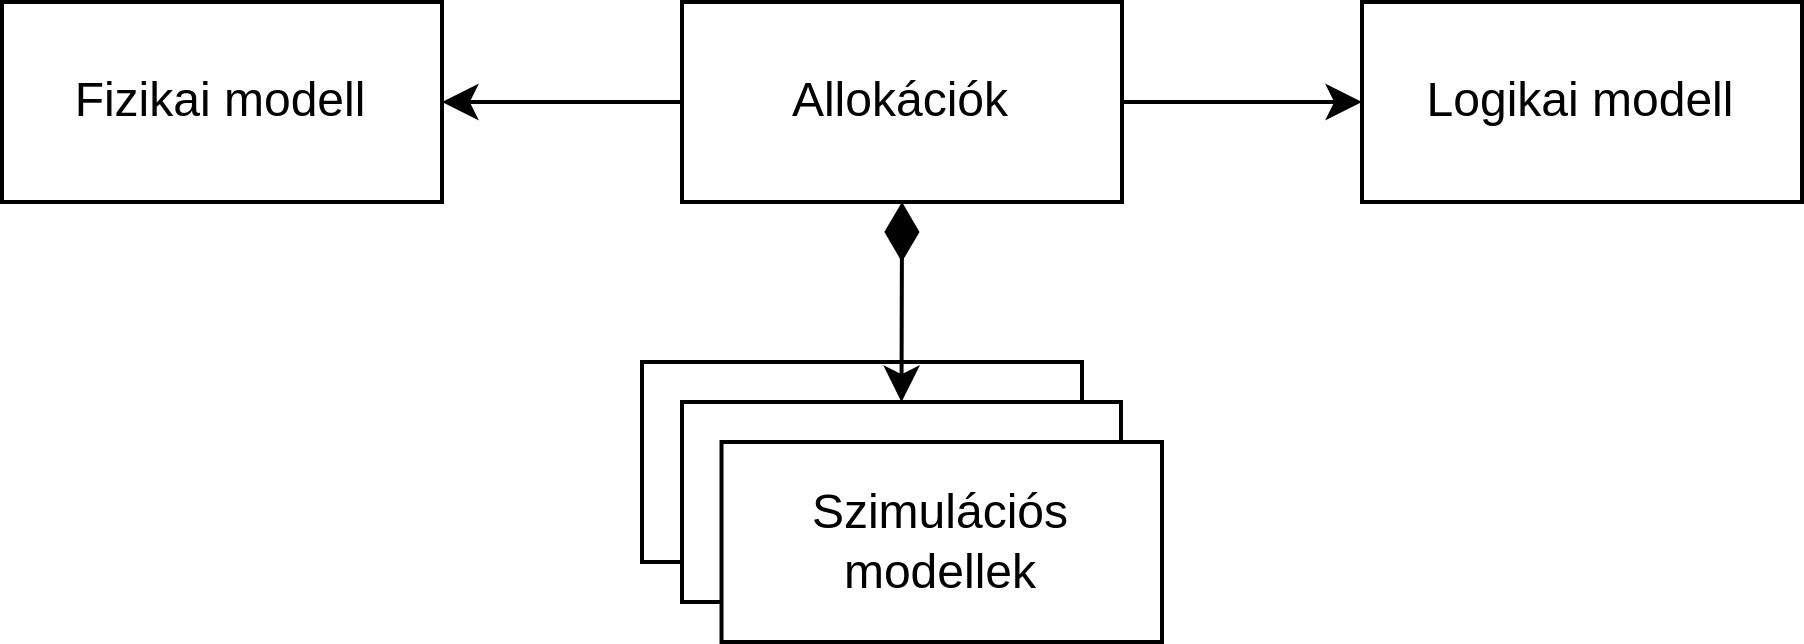
\includegraphics[width=150mm, keepaspectratio]{figures/Alapelemek.drawio.png}
            \caption{A modellek alapvető struktúrája} 
            \label{fig:Alapstruktura}
        \end{figure}

        Ennek oka, az a mögöttes gondolat, hogy a rendszereket igazából egy allokációval lehet leírni. Mivel ez a gondolat elsőre nehezen átlátható vegyünk egy példát.
        Amikor egy autót akarunk leírni, logikusnak tűnik egy \emph{Part} ként tekinteni rá --~ez a jelenleg bevett módszer is~--, mivel az \ref{sec:NyelviElemek} résznek megfelelően ez egy önmagában értelmes elem a modellben.
        Azonban amikor egy autóról beszélünk, akkor igazából valamilyen konkrét funkcióra és annak bizonyos megkötések mellett történő megvalósítására gondolunk.
        
        Nem nevezünk valamit autónak, csak mert úgy néz ki, mint egy autó, vagy ha más funkciót lát el. Ha egy óriáskerék kabinjait autókból építjük meg, akkor azokat a továbbiakban nem tekintjük autóknak, még akkor sem ha a folyamat során teljesen működőképesek maradnak, mert már nem az a funkció tartozik hozzájuk amit egy autótól elvárunk.
        Ugyancsak nem nevezzük autónak a Csillagok háborújának ikonikus homoksiklóját sem, hiába nyilvánvaló a nézőknek, hogy az autók megfelelői az adott világban. A szerkezete, amivel ezt megvalósítja eltér attól amit egy autótól elvárunk, mert forgó kerekek helyett lebeg és egy hajtómű tolja előre.

        Elsőre nehéz látni, miért fontos, hogy magát a rendszert egy másik absztrakt elemmel írjuk le, ha az eddigi megközelítés is működött. Ennek oka a későbbiekben fog látszani, mivel ez a személetváltás tette kiemelt elemmé az allokációkat a kidolgozott módszerekben.
        Tervezés közben magától értetődő gondolat, hogy a modellek finomítása attól függ milyen funkciót és milyen eszközzel akarunk megvalósítani.
        Ennek ellenére a bevett tervezői gyakorlatban az allokációkat inkább befejező lépésnek tekintik, nem a folyamat mozgatórugójának. Persze így is létrejönnek végül a modellek, de csak több iteráció után, amikor sikerült a logikai és fizikai nézeteket egymáshoz igazítani.
        A szemléletváltás után, amikor kiemelt figyelmet szentelünk ennek a megfeleltetési folyamatnak, felfedezhető, hogy ezek az információk, amelyek a fent leírt összeillesztést vezérlik, végig jelenvoltak az allokációkban, csupán figyelmen kívül maradtak a művelet helytelen szemlélete miatt.

        A szimulációs modellek is ezért kaptak helyet, az allokációkon belül, mivel azok a konkrét rendszert reprezentálják, ami a két modellnézet közti megfeleltetés.
        Ha másképpen hoznánk létre ezt a megfeleltetést a nézetek között vagy bármelyiket módosítanánk, akkor megváltoznának a szimulációs modellek is. Ebből látható, hogy ezek a modellek tényleg a rendszerhez, azaz az allokációkhoz tartoznak. Azzal, hogy az allokációk részei a szimulációs modellek egyértelművé válik melyik rendszerhez tartoznak, mert nem lehet őket elválasztani attól.

        \subsubsection{A modellek belső szerkezete} \label{sec:ModellekSzerkezete}
        Maga a módszertan javaslat három nagyobb fázisra osztható, melyek a \ref{fig:ModellStruktúra} ábrán láthatóak, különböző színekkel jelölve. Ezek egymás után, mindig az előzőre épülve jelennek meg, így a bemutatásuk is így történik a továbbiakban.
        Az ábrák konzisztensen ugyanazzal a színnel jelölik az adott fázishoz tartozó elemeket, megkönnyítendő az értelmezést.
        \begin{figure}[!ht]
            \centering
            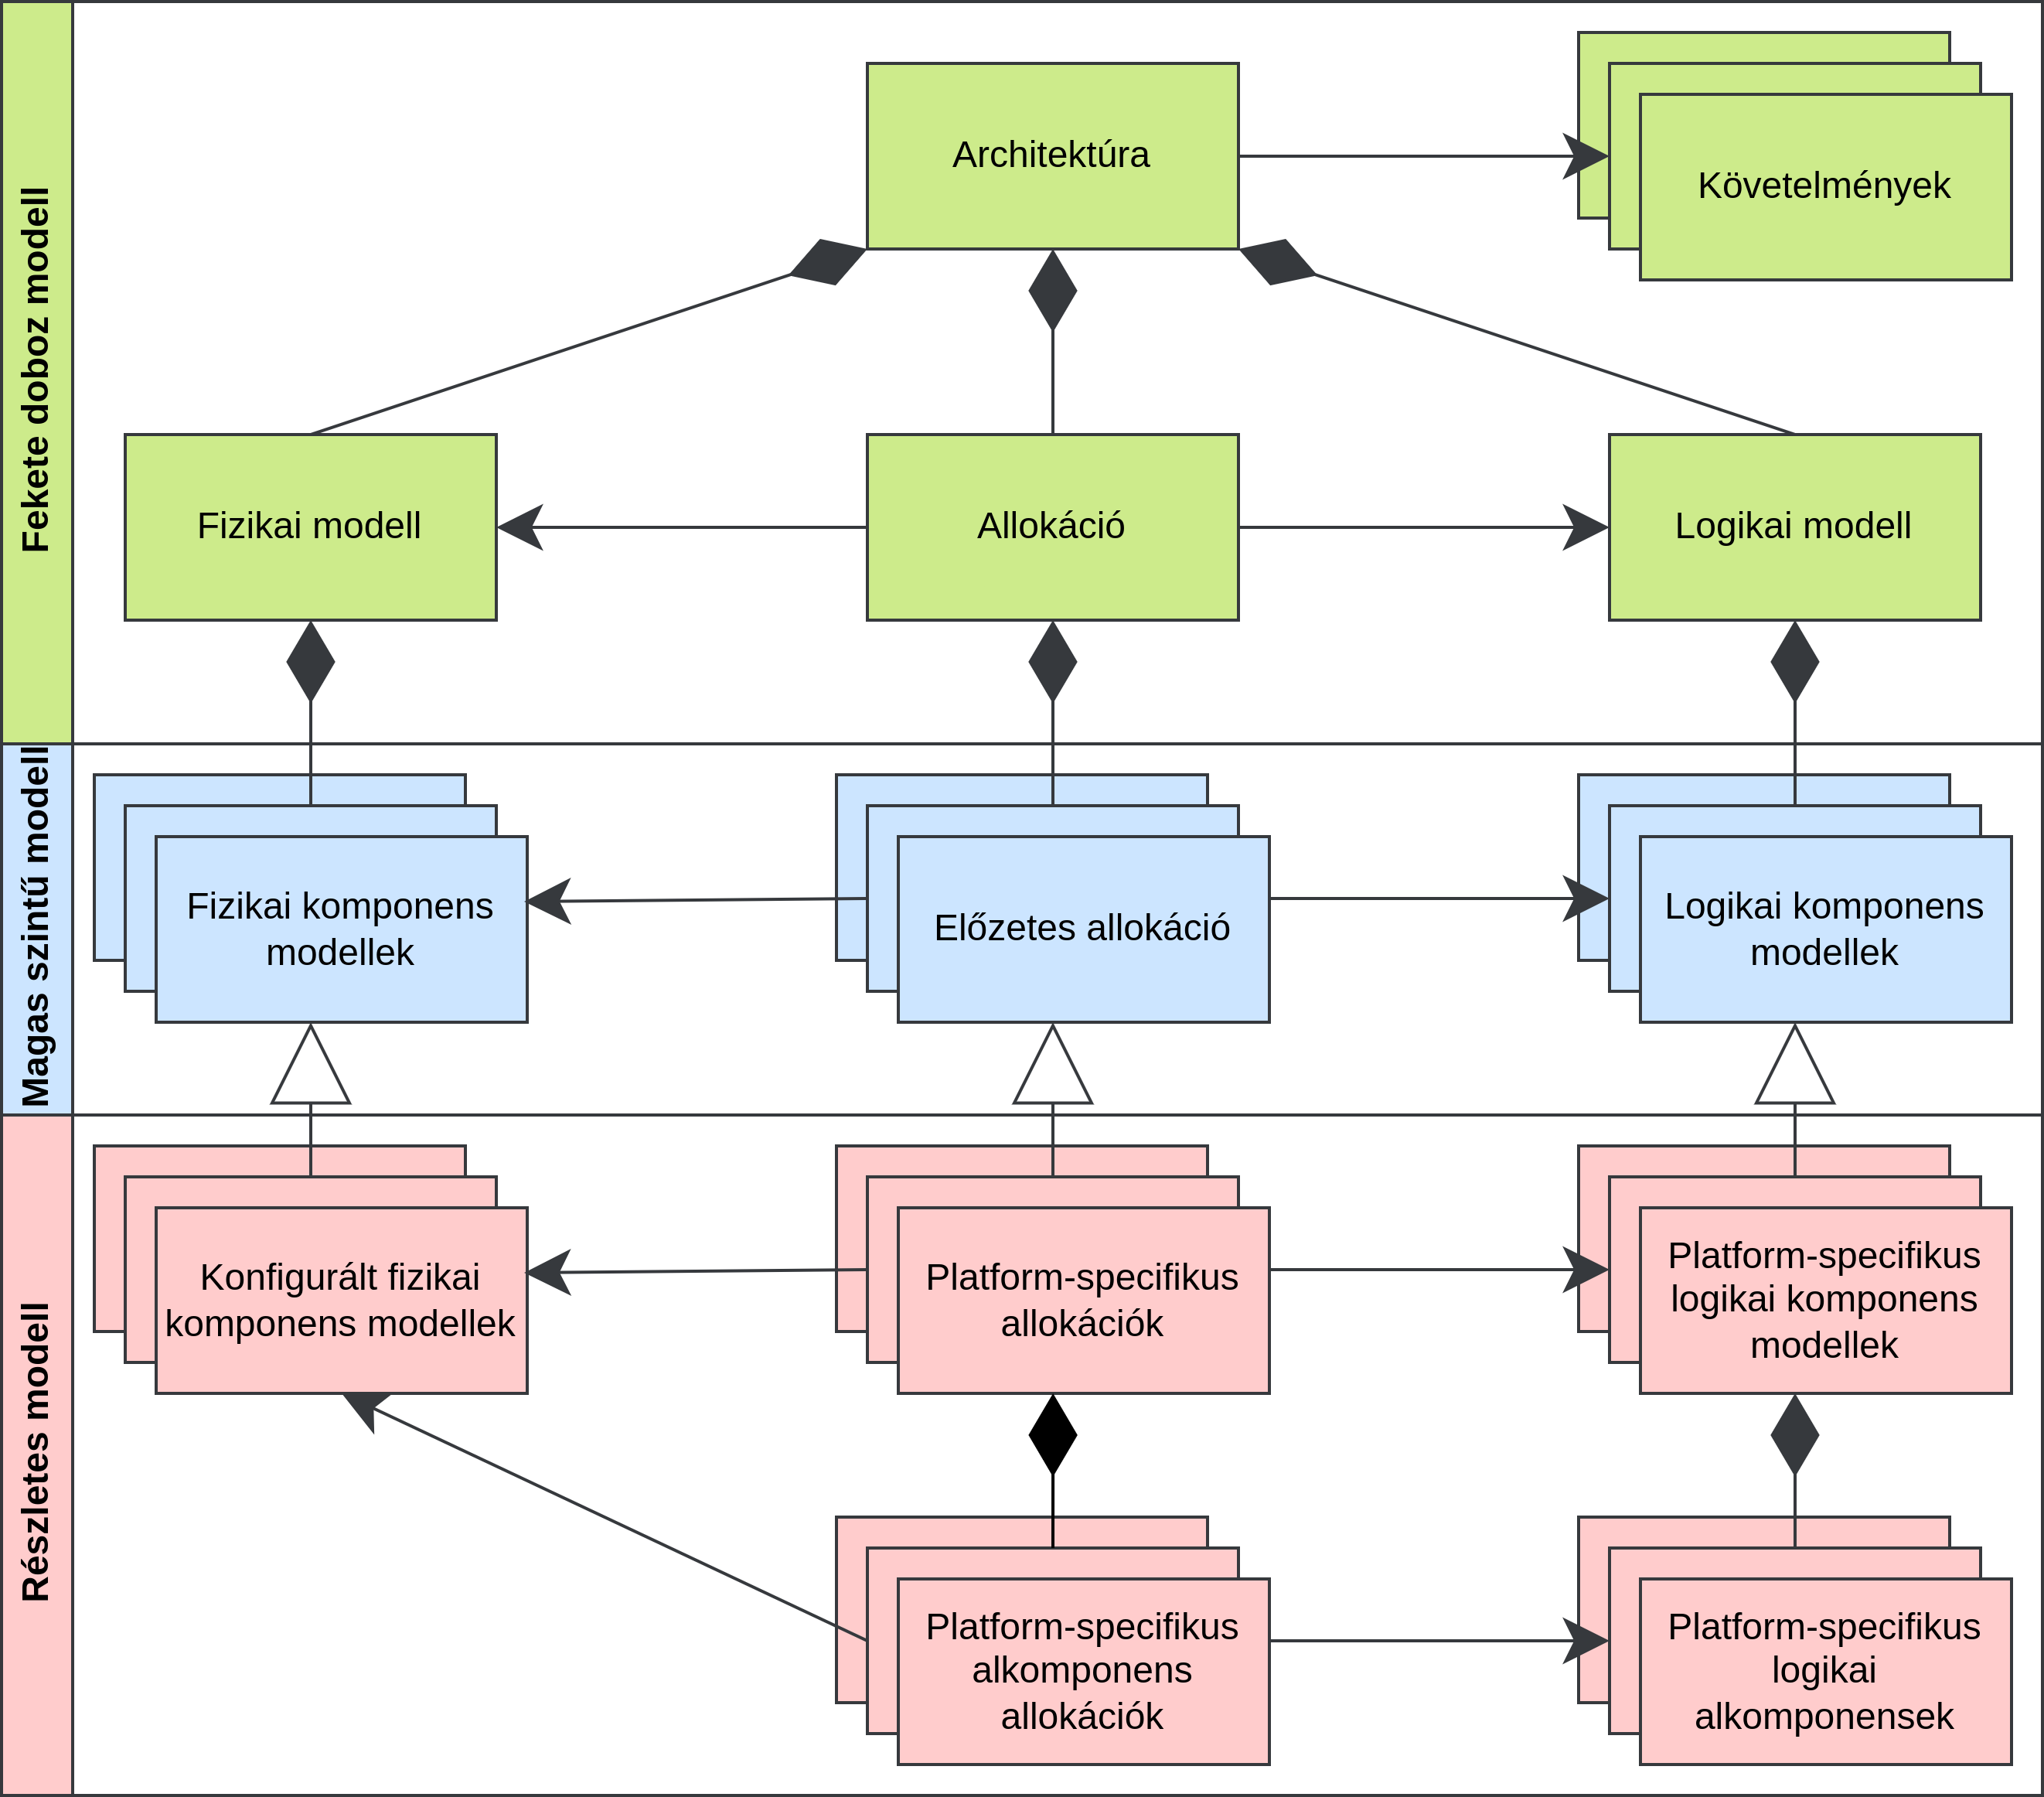
\includegraphics[width=150mm, keepaspectratio]{figures/AllocationBased2HU.drawio.png}
            \caption{A módszertan szerint készült modellek általános szerkezete} 
            \label{fig:ModellStruktúra}
        \end{figure}

        Az első fázis a \emph{Fekete doboz modell} összeállítása. Ebben a lépésben még semmilyen implementációval kapcsolatos kérdésről nem szabad dönteni, a hangsúly a rendszerrel szemben támasztott követelmények meghatározásán van.
        Az implementációs kérdések mellőzése azért kiemelten fontos, mert ha a tervezők elkezdenek egy konkrét megoldásban gondolkozni akkor az túl korán beszűkíti a lehetőségeket a megvalósítások tekintetében és elterelheti a figyelmet fontos kérdésekről a követelmények terén.
        A követelményeken kívül olyan előkészítő lépések kapnak még helyet ebben a fázisban mint a projektváz kialakítása, esetleg alkatrészkönyvtárak összegyűjtése, bár itt vigyázni kell nehogy implementációs kérdésekbe bonyolódjunk.
        A modell váza a \ref{fig:ModellStruktúra} ábrán látható a zöld színnel jelölt területen amely ennek a fázisnak felel meg.
        
        A \emph{Követelmények}-ben találhatóak a rendszerrel által teljesítendő követelmények és kapcsolódó használati esetek, míg a többi elem a projekt vázát adja meg. Ebben a vázban megfigyelhető egy gyökérelem, amely összefogja a rendszert, valamint látszik hogy ennek a rendszernek, mint egésznek kell teljesíteni a követelményeket.
        A rendszer váza tartalmazza továbbá a \ref{sec:Alapgondolatok} részben tárgyalt alapstruktúrát.
        Ezekben az elemekben találhatóak a rendszernek a környezete számára is ismert részei. Ezek az elemek a rendszer kontextusából, azaz beágyazó környezetéből ismertek.
        Például egy műhold esetében tudjuk, hogy milyen környezeti hatásoknak lesz kitéve a rendszer, milyen attribútumai vannak amelyek valamilyen érdekelt félnek fontosak, mint a tömeg és a méretek, illetve, hogy szükség lesz valamilyen vezeték nélküli kommunikációra amivel az eszköz kommunikálhat a földi irányítóközponttal. Utóbbinál fontos hangsúlyozni az implementációs kérdések mellőzését. Nem szabad belemenni olyan részletekbe, hogy rádiós, lézeres vagy valamilyen egyéb technológiát használunk majd, de az meg kell jelenjen, hogy lesz ilyen lehetőség, illetve a választandó technológia által teljesítendő követelményeket is össze kell gyűjtenünk. 
        Ezen túl ennek a váznak a szerepe, hogy a továbbiakban erre tudnak majd ráépülni a különböző modellrétegek.

        Ezután a \emph{Magas szintű modell} elkészítése következik. A logikai modellben definiáljuk, hogy milyen részfeladatokra bontva és hogyan oldjuk meg a rendszertől elvárt működés biztosítását.
        A fizikai modellben megadjuk milyen alrendszerek és alkatrészek segítségével biztosítjuk ezeknek a logikai feladatoknak az elvégzését.
        Végül az \emph{Előzetes allokációkkal} hozzárendeljük a feladatokat ezekhez a fizikai komponensekhez.
        
        A javasolt módszertan szempontjából legfontosabb részlet, hogy ezek az \emph{Előzetes allokációk} egyetlen logikai elemet több fizikaihoz is hozzárendelnek. Ez a végleges modellben már nem lenne előnyös, mert mindig pontosan egy felelősre van szükség egy adott feladat végrehajtásánál, de a magas szintű terveknél éppen ezt szeretnénk elérni.
        Ennek oka, hogy a fizikai és logikai nézeteket nem véletlenül választottuk külön, az egyes vetületekben a komponensek határai tipikusan eltérnek, átlapolódnak.
        Ha ez nem így lenne, akkor valószínűleg nem sikerült rendesen elválasztani a két nézetet, tehát ez egyik túl nagy mértékben meghatározta a másikat vagy már túlzottan belemerültünk az implementáció részleteibe. Mindkét eset könnyen vezethet szuboptimális megoldásokhoz és nehezen átlátható modellekhez. (Lásd: \ref{sec:LogFiz}. követelmény)
        
        A célunk, hogy ezeket a többszörös allokációkat és mögöttes jelentésüket fel tudjuk használni a modell további finomítása során. Ez a rejtett információ az, amely korábban sokszor iteratív finomítással került feltárásra, pedig helyes allokációkkal és azok vizsgálatával könnyen átlátható.
        A következő fázis előtt fontos kitérni arra, hogy mi is okozza pontosan a többszörös allokációkat, illetve milyen információt hordoznak a későbbi lépések számára.
        
        A fő ok, hogy a kérdéses logikai feladatot több fizikai komponens együttes munkája képes ellátni. Ebben az esetben ezt a feladatot tovább kell bontani az alapján, hogy milyen részfeladatokat melyik komponens valósít majd meg.
        Azért fontos, hogy ez a lebontás ne a magas szintű modellben történjen, mert annak feladata az adott probléma minél pontosabb megértése és hatékony megoldása, nem a konkrét implementáció elkészítése.
        Ha már ezen a szinten elvégeznénk a feladatok felosztását a fizikai komponensek függvényében, akkor az megnehezítené a modell átlátását, mert megfosztana minket a hierarchikus tervezési módszerektől amelyeket a \ref{sec:Hierarhia}. követelmény kifejtésében tárgyaltunk.
        
        A másik lehetséges ok a biztonságkritikus rendszerekkel szembeni követelményekből és azok teljesítéséből adódik. Név szerint a redundáns alrendszerekből. Ha csökkenteni akarjuk egy alrendszer meghibásodásának esélyeit akkor gyakran az egyetlen ésszerű megoldás az, ha több példányt is beépítünk belőle a rendszerbe, amelyek külön-külön is képesek ellátni a feladatukat.
        Ennek előnye, hogy annak jóval kisebb az esélye, hogy több is meghibásodik a kérdéses rendszerből\footnote{Ez az állítás csak független hibaokokat feltételezve érvényes. Ha ezt nem feltételezhetjük, akkor diverz tervezéssel védekezhetünk, ahol a duplikált alrendszerek nem pontos mások. Csak a velük szembeni követelmények azonosak, az implementáció minél eltérőbb, minimalizálandó az összefüggő hibaokokat. Például hiába használunk több GPS modult helymeghatározásra, ha nem az egyes modulok hanem maga a GPS hálózat válik működésképtelenné, akkor a redundancia önmagában nem nyújt védelmet.}, így tovább növelhettük a rendszer megbízhatóságát.
        A redundancia implementálása szintén későbbi lépésekben célszerű, felesleges bizonyos részfeladatok duplikálásával bonyolítani az áttekinthetőséget célzó magas szintű terveket, amikor ennek oka a konkrét implementációval szemben támasztott elvárások.

        A harmadik fázis a \emph{Részletes modell} megalkotása.Ebben a lépésben finomítjuk tovább a fentiekben leírtak szerint a modellt, hogy megkapjuk a már említett egy-egy kapcsolatokat létrehozó allokációkat.
        A \ref{fig:ModellStruktúra} ábrán látható, hogy ez esetben az új elemeket nem tartalmazza az eggyel korábbi lépés, hanem az új elemek \emph{specializálják} a magas szintű komponensmodelleket.
        
        Ennek oka, hogy a feladatoknak az egyes alkatrészek között több lehetséges felosztás is lehetséges. Azzal, hogy egy specializációval leválasztjuk ezt a réteget a magas szintű tervekről, lehetőségünk van több leszármazottat definiálni, amelyek a szimulációs modellek segítségével összehasonlíthatóak lesznek teljesítmény szempontjából.
        A több lebontás kapcsán gondolhatunk arra, hogy hogyan osztunk meg szoftverkomponenseket több processzor között a fogyasztás, válaszidő vagy pontosság alapján optimalizálva. De ugyanígy lehet szó arról, hogy a magas szintű modellben csak azt határoztuk meg, hogy egy adott gyártó melyik termékcsaládjából választunk például villanymotort egy adott feladatra, amely a vezérlés szempontjából már elegendő magas szinten, és csak a specializáció után választunk konkrét típust, amikor már pontosabb adataink vannak a várható terhelésről.

        Maga a lebontás először a logikai elemek dekompozícióját jelenti a fizikai komponensek alapján, ezzel létrehozva a \emph{Platform-specifikus logikai komponens modelleket}.
        A következő lépés a fizikai komponensek konfigurálása. Ez a különböző paramétereik meghatározását jelenti úgy, hogy ezzel készek legyenek a megfelelő feladatok ellátására.
        Ez lehet akár egy szabályozó paramétereinek hangolása, a memória kiosztása egy mikroprocesszoron, de konfigurálható logikai áramkörök esetében a konkrét áramkörök megtervezése és a megfelelő hardver erőforrások hozzárendelése is.
        Végül elkészítjük a \emph{Platform-specifikus allokációkat} is, amelyekben alacsonyabb szintű allokációkkal teremtjük meg a már említett egy-egy kapcsolatokat a \emph{Platform-specifikus logikai komponens modellek} és a \emph{Konfigurált fizikai komponens modellek} között.

        \subsubsection{A fejlesztés menete} \label{sec:flow}
        Az előző fejezetben már látható volt, hogy milyen főbb lépésekre tagolódig a rendszertervezés a javasolt módszerek használatával, de a modell szerkezete csupán egy egyszerűsített képet ad erről.
        Ebben a részben ez a folyamat kerül részletesebb bemutatásra.
        
        Maga a fejlesztési folyamat a \ref{fig:Folyamat} ábrán látható. Az ábra színezése megfelel a korábbiaknak elősegítendő a tájékozódást.

        Az első fontos észrevétel a szimulációs modellek újbóli megjelenése. Míg a \ref{fig:Alapstruktura} ábrán látható, hogy az allokációk szimulációs modelleket tartalmaz(hat)nak, míg a \ref{fig:ModellStruktúra} ábrán ezek nem voltak jelölve.
        Ez a változtatás csupán az ábra átláthatósága miatt történt, ezek a modellek továbbra is be vannak ágyazva az allokációkba, csupán az egyébként is összetett ábráról lettek lehagyva a megértés megkönnyítésének érdekében.

        \begin{figure}[!ht]
            \centering
            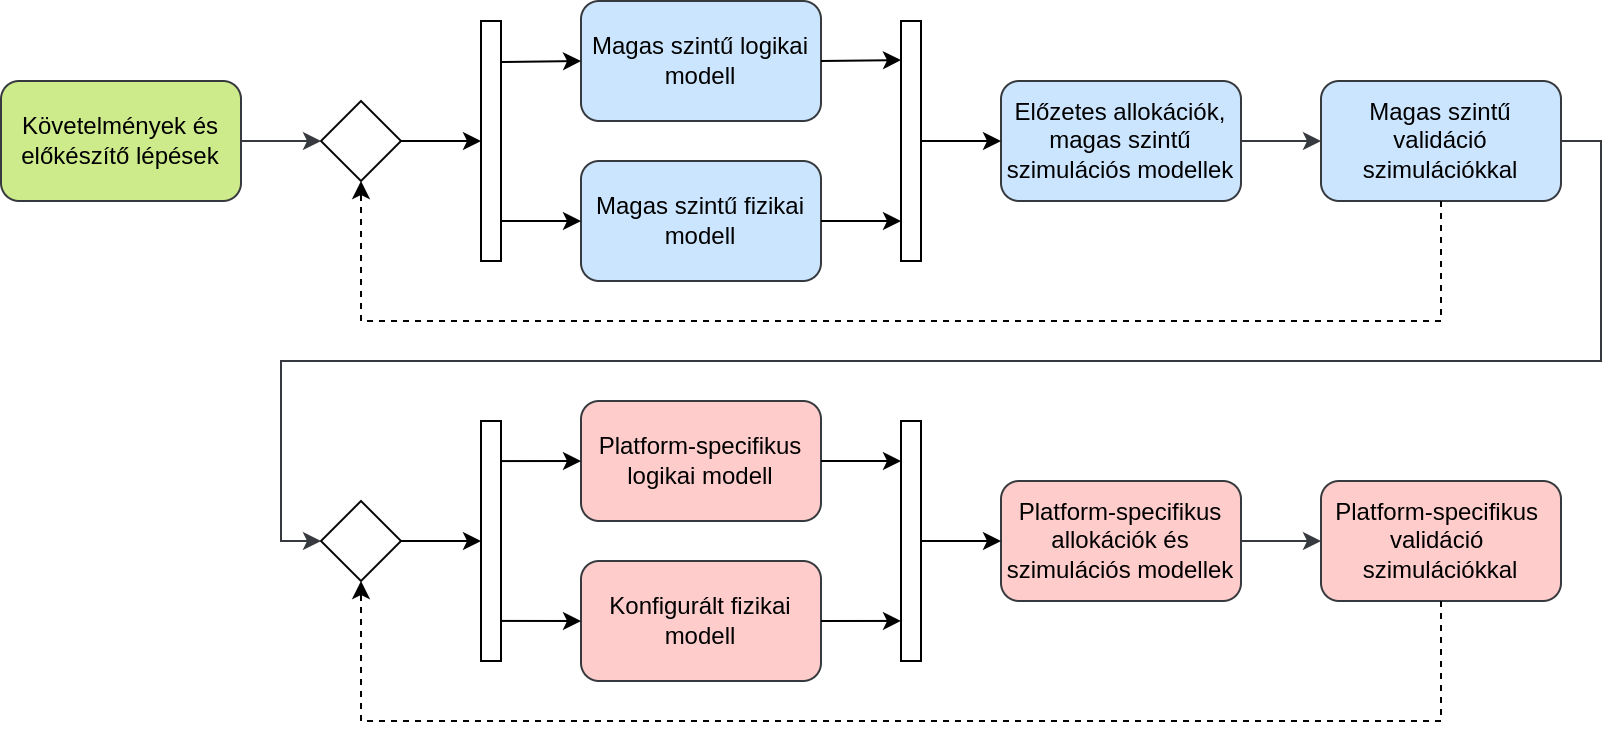
\includegraphics[width=150mm, keepaspectratio]{figures/ParalelAllocationBasedFlowHU.drawio.png}
            \caption{A fejlesztési folyamat menete} 
            \label{fig:Folyamat}
        \end{figure}

        Visszatérve a fejlesztés menetére, látható, hogy az első fázis a jelenlegi módszerek mellett egyetlen lépést igényel csak. A követelmények összegyűjtése és a javasolt módszertan által megkövetelt alapstruktúra létrehozása történik meg, a további munka előkészítéseként.
        
        A következő két fázis meglehetősen szimmetrikus, így azokat vizsgálhatjuk együtt. Először a logikai és fizikai modellek finomítása következik. Ez a két lépés haladhat párhuzamosan, mert az előző fázisokból szerzett információk alapján mindkét modell finomítása elkezdhető, de meg kell említeni, hogy a fizikai modell aktuális bővítésének befejezéséhez gyakran szükséges a logikai modell elkészítése. Erre jó példa a \emph{Konfigurált fizikai komponensek} esetén egy mikrovezérlő memóriatartományának felosztása.
        Ugyanakkor a redundáns alrendszerek duplikálása nem igényli a pontos logikai modellt, így azt célszerű azzal párhuzamosan végezni.
        
        A folyamatábráknál az ilyen párhuzamosság jelölés azt jelenti, hogy a feladatok végrehajtásának sorrendje nem ismert, tehát nemcsak valódi párhuzamosságot jelöl a fenti ábra, csak pontos sorrend nélkül végezhető feladatokat.
        A kidolgozott módszertan javaslatban ez a sorrend az alkalmazott tervezési irányelvektől függ. Így megengedett top-down, bottom-up és kevert módszerek alkalmazása is. Fontos megemlíteni még az autóiparban egyre inkább elterjedő platformalapú módszereket, ahol a fizikai modell megelőzi a logikait, mert annak alapja többnyire már adott a rendszer tervezése előtt, lényegi változtatás csak az utolsó, konfigurációs fázisban történik rajta.
        Egy fázisokra bontott, és adott lépésben megengedőbb módszertan éppen azért célravezető, mert a lehető legkevésbé köti meg a módszer alkalmazóinak kezét az alkalmazandó tervezési irány tekintetében, elősegítve a széleskörű alkalmazhatóságát.
        
        Ha elkészült a két modellnézet, akkor létrehozhatjuk az adott szinthez tartozó allokációkat és ezek alapján elkészítjük az új, részletesebb szimulációs modelleket.
        Végül mindkét fázisban felhasználjuk a szimulációs modelleket, hogy validálhassuk az új modelleket mielőtt továbblépnénk a következő fázisra. Természetesen nem csak szimulációt használunk validációra, de a javaslatok újdonsága ezeknek a technológiáknak a támogatása.
        
        Amennyiben a validáció nem sikeres egy új iterációban megismételjük az adott fázist. Fontos, hogy ez az iteráció a validáció elbukásának következménye, a korábbi módszerekben megjelenő iteratív illesztést a logikai és fizikai modellek között már feloldottuk, ezt a típust pedig nem lehet.
        Ha sikeres volt a fázis végén a validáció, akkor tovább lépünk a módszertanban.
        
        Ezeknél a validációs méréseknél van lehetőség végrehajtani a \ref{sec:ModellekSzerkezete} részben említett kiértékelést a különböző implementációk között, mivel itt egyébként is futtatunk ilyen méréseket a továbblépés előtt.
        Ezen túl meg kell említeni, hogy a javasolt módszerek alkalmazhatóak az egyes alrendszerek kapcsán is. Az első fázis itt az adott alrendszerre vonatkozó követelmények összegyűjtése, ezután pedig a módszertan lépései ugyanúgy ismételhetők az adott komponensen belül.
        Szintén alkalmazható ez a módszer a rendszer kontextusának modellezése során, ilyenkor gyakorlatilag egy olyan modellt alkotunk meg, amelynek a rendszerünk csak egyetlen eleme, célja pedig a környezeti elemek egymással és a rendszerrel való kölcsönhatásainak leírása.
        Ilyen modelleket minden módszertan használ a fejlesztés elején (Lásd: \ref{sec:KorabbiModszerek} rész), sajnos ennek a lépésnek a részletes vizsgálatára a dolgozat kereteiben nem volt lehetőség.

        \subsubsection{A könyvtárak szerkezete és használata}
        Ahogy az a \ref{sec:Ujrahasznalas}. követelménynél is olvasható volt, a tervezés során gyakran felmerül az igény az egyes komponensek újrahasználására, esetleg külső beszállítótól való beszerzésére.
        Ennek megkönnyítésének érdekében a módszertannak támogatni kell komponenskönyvtárak létrehozását és használatát is.
        A módszertanhoz kidolgozott könyvtárstruktúra a \ref{fig:Konyvtar} ábrán látható.
        \begin{figure}[!ht]
            \centering
            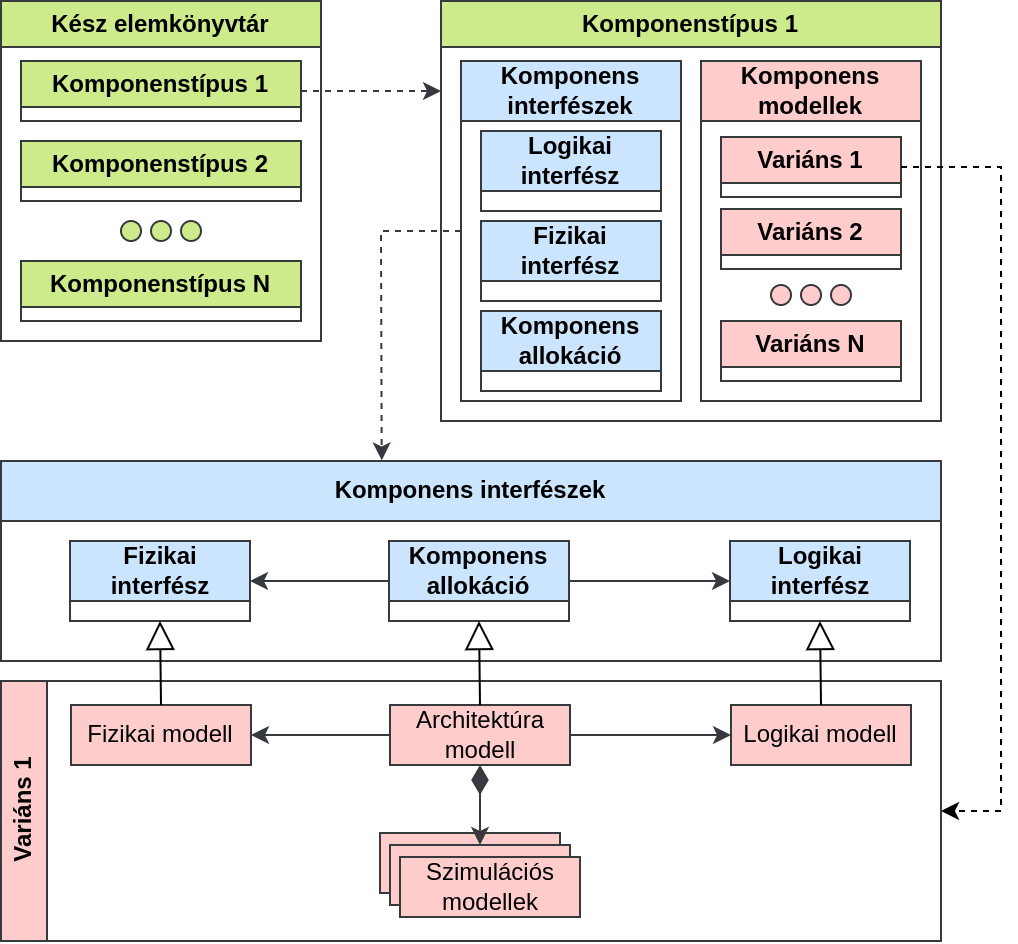
\includegraphics[width=150mm, keepaspectratio]{figures/InterfaceParts.drawio.png}
            \caption{A komponenskönyvtárak szerkezete.} 
            \label{fig:Konyvtar}
        \end{figure}

        A könyvtáron belül komponenstípusok vannak. Ezekbe a kifelé --~a paramétereiket leszámítva~-- azonosan megjelenő komponensek kerülnek csoportosításra, mint például szervomotorok, egyenáramú motorok, stb.
        Egy komponenstípuson belül definiálva van egy általános komponens-interfész, amely egy alapvető modell, amely a külvilág által látható elemeket tartalmazza a komponenstípusra vonatkozóan. Ez az alapvető fizikai és logikai modellből valamint az azokat összekötő allokációs típusból áll.
        
        Az allokációhoz azért célszerű külön típust bevezetni, mert megadható benne, hogy milyen típusú elemeket képes allokálni, így csökkentve a hibalehetőségeket.
        
        Ezenkívül minden konkrét komponenshez tartozik egy-egy ilyen komponens-specifikus típus is, amely \emph{specializálja} az általános verziót.
        
        Ennek azon túl, hogy illeszkedik a kidolgozott módszertanba két előnye van.
        Először is a specializált allokációban szűkíthetjük a végekre vonatkozó típuskövetelményeket, hogy csak az összetartozóakat fogadja el a konkrét komponensmodellekből, ezzel is csökkentve a modellezési hibák előfordulását.
        Másodszor pedig, az azonos típusú komponenseknek a legtöbb esetben csak apróbb eltérések jelentkeznek a szimulációs modelljeiben, a legjellemzőbb, hogy csak paramétereikben térnek el.
        
        Ha a megfelelő szimulációs modellvázak szerepelnek az általános allokációban, akkor a konkrét típusnál elég a paramétereket felülírni és azt a néhány kisebb módosítást redefiniálni, ha ez szükséges.
        
        Ezzel csökkenthető a kódduplikáció, megkönnyítve a könyvtárak karbantartását. Ez azért is fontos, mert a \ref{sec:fmi}-ben megismert FMI szabvány által definiált csomagok, amelyeket a gyártók biztosítani szoktak a megrendelőiknek szimulációs célra szintén paraméterezhetőek, illetve relative nagy méretűek a rendszermodellekhez képest.
        Ha tehát ezekből minél kevesebbet kell a könyvtárral együtt tárolni, akkor azok mérete radikálisan csökkenthető.

        \subsubsection{Szimulációs modellek használata}
        Mivel a módszerek kidolgozásánál külön cél volt a szimulációs technológiák integrálása, ezért tekintsük át az ezekre vonatkozó részeket.
        
        A szimulációs modellek rendszermodellen belüli reprezentációival kapcsolatos elvárások a \ref{sec:SzimIntKov}. követelménynél olvashatóak. A legfontosabb követelmény, hogy több szimulációs modellt is támogasson a módszertan egy adott komponenshez, teljesül, mivel több is hozzárendelhető az allokációkhoz.
        Ezeknek a modelleknek a finomítása ráadásul folyamatosan történik a módszertan folyamán, a rendszerrel együtt fejlődnek és szerves részét képzik a fejlesztési folyamatnak, a tervezői döntéshozásnak.
        
        Ezzel elérhető a \ref{sec:mbseElonyei} és \ref{sec:szimElonyok} részekben leírt minden fejlesztési fázisban jelenlévő V\&V tevékenység és gazdaságosság, mivel a módszer a lehető legkorábbi fázisban kiszűri a koncepcionális vagy implementációs hibákat.

        Azzal, hogy a nagyobb fázisokban hierarchikusan helyezkednek el az egyes allokációk, támogatható, hogy egy magasabb szinten lévő modell hivatkozzon az általa tartalmazottakra, így a szimulációs modellekre is kiterjesztődnek a \ref{sec:Hierarhia}. követelménynél tárgyalt hierarchikus módszerekre vonatkozó előnyök.
        
        Mivel a hierarchiában minden szint több szimulációs modellt támogat, így hierarchikus szimulációs modellek használatával még egyszerűbbé válik a különböző részletességű szimulációs modellek készítése, mivel a az alkomponensek esetén elég a használt szimulációs modellek hivatkozásait redefiniálni.

        \subsubsection{Kontextus modellezés}
        A rendszertervezési módszertanokban (Lásd: \ref{sec:KorabbiModszerek} rész) rendszerint a rendszer modellezése mellett nagy hangsúlyt helyeznek annak kontextusának, azaz beágyazó környezetének a modellezésére. Fontos tehát ezt a területet is részletesen megvizsgálni, hogy minél közelebb kerülhessünk egy teljes, gyakorlatban is jól alkalmazható módszertanhoz.

        A rendszer kontextusa az, ami meghatároz számos követelményt, illetve azt, hogy a rendszer hogyan lép interakcióba a környezetét alkotó elemekkel.
        Ezek azok a kapcsolódási pontok és követelmények, amelyek a már bemutatott módszerekben a fejlesztés első fázisában jelentek meg, tehát nem meglepő, hogy ez az alfejezet ahhoz a lépéshez tartalmaz kiegészítéseket.
        
            \paragraph{A nézetek fontossága}
            Elsőre kérdéses lehet, hogy a kontextusmodellnél is szükséges-e a logikai és fizikai nézetek elválasztása.
            A válasz igen, de a megértéséhez célszerű egy konkrét példát venni.
            
            Ha egy műholdat tervezünk, akkor szeretnénk vele kommunikálni a földről. Ez történhet egyetlen földi állomásról is, de van, hogy jóval többet akarunk kommunikálni, mint amennyit egyetlen földiállomás lehetővé tenne. Ilyenkor erre a célra használhatunk több földiállomást is, amelyek azonban lehet hogy nem egyformák. Ilyenkor a fizikai modellben lehet hogy teljesen más frekvenciasávon, sávszélességen és modulációval valósul meg a kapcsolat, de logikailag nincs feltétlenül különbség.
            Ilyenkor azt szeretnénk, hogy a logikai modell a lehető legegyszerűbb maradjon, de a fizikaiban megjelenjenek ezek a részletek is, mivel ezek fontosak a fejlesztés szempontjából.

            A szétválasztás azért is fontos, mert a rendszer esetében is jellemzően más-más szakemberek dolgoznak ezeken a területeken. Ez valószínűleg a kontextusmodell esetében is így van, de ha mégsem, akkor is célszerű úgy elkészíteni ezt a modellt, hogy az könnyen használható legyen a továbbiakban.

            \paragraph{Analógiák az egyes fázisok során}
            Azért fontos külön foglalkozni a kontextusmodellel, mert jellemzően nem pontosan ugyanaz a folyamat szükséges az elkészítéséhez, mint a rendszermodell esetében, de a főbb gondolatok továbbra is azonosak.
            Vegyük végig a korábban bemutatott fázisokat a kontextusmodellre nézve és vizsgáljuk meg, hogyan alkalmazhatóak ehhez a modelltípushoz.

            A kontextus \emph{Fekete doboz modelljének} elkészítése során a már ismert követelményeket ugyanúgy felvesszük, azonban a logikai és fizikai modellek esetében nem jelennek meg a rendszernél látott külvilág számára ismert elemek.
            Ennek oka, hogy a kontextus maga is egy rendszer, méghozzá zárt. Nincsenek tehát, olyan kívülről ismert elemei mint magának a megtervezendő rendszernek. Ha lennének ilyen elemei, akkor azok a kontextus kontextusához kapcsolódnának és ez a folyamat talán sosem érne véget.
            Az, hogy hol állunk meg, mi tartozik a kellően részletes kontextusmodellhez és mi az ami már felesleges részlet, természetesen már egy tervezői döntés. A javasolt módszerek nem adják meg hol húzzuk meg ezt a határt, csupán a létét követelik meg, hogy a valódi rendszerek modellje is kezelhető mértékű maradjon, ezzel a zárt világ szemlélettel.

            A rendszerünk célja, hogy valamilyen formában interakcióba lépjen a környezetével. A kontextusmodell megadja, hogy milyen feltételezésekkel élhetünk majd a tervezés során, illetve milyen követelményeknek kell megfelelnie a rendszernek, hogy megfelelő módon interakcióba a környezetével.
            Megfordítva, a rendszerünkre vonatkozó követelmények azok a feltételezések, amelyekkel a beágyazókörnyezet él a rendszerünk kapcsán. Mivel a környezetünk feltételezéseit rendszerint nem tudjuk megváltoztatni, így számunkra követelmény, hogy megfeleljünk ezeknek a siker elérése érdekében.

            A \emph{Magas szintű modell} szintjén kezdjük el kibontani a kontextusmodellt. Ebben az esetben nem funkciók és alkatrészek jelennek meg, hanem a rendszer és kontextusának elemei, valamint az egyes elemek közti kapcsolatok.
            A cél a kontextust addig finomítani ebben a lépésben, hogy minden fontos szereplő megjelenjen.
            
            A korábbi műholdas példában a rádiós kapcsolatok esetén például foglalkoznunk kell a különböző zajokkal.
            Ezek a logikai modellben elég ha zajként megjelennek, mivel a szerepük itt az, hogy a feladatoknál később foglalkozzunk a zajszűréssel.
            Ellenben a fizikai modellnél szeretnénk lebontani ezt szűkebb csoportokra. Például származhat a zaj más kommunikációs eszközökből, lehet háttérsugárzás, de akár aktívabb naptevékenység is. Ezek tipikusan másképpen viselkednek és másképpen is lehet védekezni ellenük a fejlesztés során, hiába ugyanaz a feladat logikailag.

            A \emph{Részletes modellben} a konkrét implementációhoz kapcsolódó elemekkel bővítjük az eddigi modellt. Ide tartoznak például, hogy egy rádiós kapcsolat milyen paraméterekkel valósul meg a rendszer és kontextusa között.
            Milyen frekvenciasávot és modulációt használunk, milyen protokollt kell betartanunk. Ez az a szint, amely hasonló rendszerek esetén is eltérhet, például két különböző műholddal szemben hasonlóak a magasszintű elvárások, azonban a konkrét feladatuk már számos különbséget határoz meg, amelyek eltérő kontextusmodellt eredményeznek.
            Azzal, hogy a kontextusmodellben is elválasztjuk a ezeket a szinteket, elősegítjük, hogy ezek a modellek is részben újrahasználhatóak legyenek.

            Feltéve, hogy a műholdas példát egy műholdgyártó cég szemszögéből nézzük, szeretnénk, ha lenne egy stabil alapunk a termékeink tervezésénél. Az első két fázis nagyrészt megegyezik az egyes megrendelések között, ha egyszer jól elkészítjük ezeket a modelleket, akkor az újrahasználásuk nem csak gyorsabbá, de biztonságosabbá teszi a tervezési folyamatot, mert a jövőben nem maradhatnak ki a már ismert tényezők a modellből.
            Az egyes megrendelésekben csak a \emph{Részletes modellt} kell mindig újra elkészíteni a konkrét igények kapcsán, de ez már ráépül a meglévő, biztos alapokra.
            
            Ez a megoldás hasonló az autóiparban jellemző platformalapú módszerekhez, mert csak a pontos feladathoz kell igazítani a meglévő eszközöket, bár ebben az esetben inkább egy keretrendszerről beszélhetünk az adott feladat kapcsán.
            
            \paragraph{Az allokációk fontossága}
            A rendszertervezés során kiemelt figyelmet kaptak az allokációk. A kontextusnál ez a szerep továbbra is megmarad, mivel a nézeteket továbbra is össze kell kötni és a szimulációs modelleknek is meg kell jelenni a modellben.

            Továbbá láttuk, hogy továbbra is jelen van egy folyamatos finomítás a módszerekben kibontandó hierarchiákkal, amelyek kezelésére szolgál az általam bevezetett allokációkon alapú modellezési szemléletet.

            Az allokációk szerepe azért is fontos továbbá a kontextusmodellben, mert azt szeretnénk, hogy a rendszermodell pontosan illeszkedjen a kontextusmodellbe, amihez elengedhetetlen az azonos struktúra.

            \paragraph{A rendszer megjelenése}
            Felmerülhet az a kérdés, hogy hogyan jelenik meg maga a rendszer, amelyre több válasz is adható.
            A kérdés onnan ered, hogy a rendszerünk nem feltétlenül egyetlen elem, hanem több különálló egység, azaz rendszerek rendszere.
            Ez kiemelten fontos elosztott kiberfizikai rendszerek esetén, ahol egy-egy eszköz tipikusan limitált képességekkel bír és több egység együttműködésével oldható meg egy feladat.
            Ilyenkor a rendszer elemei egyben egymás kontextusát is alkotják.

            Ha tényleg egyetlen elemünk van, akkor természetesen ez egy egyszerű kérdés, a rendszert egy elem reprezentálja.
            Jó megközelítés lehet ez akkor is, ha egy adott csapat készíti el az összes komponenst, mert így először a teljes rendszerre összpontosíthatnak és az így feltárt követelményeket később felhasználhatják a rendszer komponenseinek lebontásánál.
            Ez a megközelítés akkor is jól működik, ha előre nem tudjuk, hogy szükség van ilyen lebontásra, vagy nem ismert pontosan, milyen lebontásra lesz szükség.

            Ha viszont előre ismerjük a lebontást, vagy a komponenseket több külön csapat fejleszti majd, akkor felvehetjük előre az egyes komponenseket is az előbb bemutatott hierarchia alkalmazása nélkül is. Így minden alrendszernek elkészítve a kontextusmodelljét.

            A két módszer között nincs egyértelmű sorrend, az alkalmazásuk inkább az adott projekttől és a fejlesztő szervezet struktúrájától, esetleg saját konvencióktól függ, az is elképzelhető, hogy ezeknek egy kombinációját használjuk és még több hierarchiát vezetünk be.
            Ez csupán egy kitekintés, amely modellezési javaslatokat vezet be a módszerek esetleges alkalmazóinak.

            \paragraph{A rendszer fejlesztése a kontextusmodell alapján}
            A kontextusmodellt elsősorban a rendszerek fejlesztésének elősegítéséhez alkotjuk meg a kezdeti lépések között, de látható, hogy a rendszer tervezésének első lépéseivel együtt jön létre.

            Azzal, hogy a fentiek szerint a rendszermodellel összhangban álló struktúrát alkalmaztunk ehhez a modellhez is, lehetőségünk nyílik arra, hogy a kettőt szorosabban összefűzzük, hiszen két azonos modell elkészítése a rendszerről felesleges lenne, csupán hibalehetőségeket vinne a tervezési folyamatba.

            Ehelyett megtehetjük, hogy a rendszernek egyetlen modellje van, amely be van ágyazva a kontextusmodellbe. Ez a továbbvitele annak a korábbi gondolatnak, hogy a kontextusunk egy ugyanolyan rendszer, mint a miénk, csupán egy zárt világban. Ennek a világnak az egyetlen része, amit tetszőlegesen alakíthatunk, az a saját, általunk tervezett rendszer, ami így folyamatosan kerül kibontásra, a kontextusmodellel együtt.

            A módszer előnye, hogy nincs két független modell a rendszerünkről, szóval ezek nem is kerülhetnek inkonzisztens állapotba, a nyomonkövethetőség sokkal egyszerűbben garantálható, mit két külön modell esetén.

            \paragraph{A szimulációk szerepe}
            A szimulációk szempontjából a kontextusmodellnek kiemelt szerepe van. Mivel a javasolt módszerek szempontjából kiemelten fontosak a szimulációk, így célszerű ezt a szempontot is megvizsgálni a kontextusmodellek kapcsán.

            A szimulációk lényege, hogy a rendszerünk egy virtuális megfelelőjét egy virtuális környezetben tudjuk vizsgálni, ezzel elkerülve, vagy legalább csökkentve a fizikai teszteléssel járó időszükséglet és költségek mértékét.

            A kontextusmodell az, amely a teljes rendszerre nézve leírja ezt a virtuális környezetet, tehát ha nem csak egy-egy komponenst akarunk így validálni, akkor elengedhetetlen egy ehhez megfelelő kontextusmodell elkészítése.

            Bár a rendszer tervezésénél a \emph{Fekete doboz modell} elkészítésénél még nem alkalmaztunk szimulációkat, a kontextusmodellezés esetén mégis hasznos lehet.
            
            Vegyük a korábbi műholdas példát. A különböző rádiós berendezések költségesek így szeretnénk minél kevesebb ilyen alrendszert felhasználni a műholdunkhoz, de legalább annyi kell, hogy megbízhatóan kommunikálhassunk a műholddal a szükséges gyakorisággal.
            A különböző kommunikációs-alrendszer konfigurációkat szimulálva meghatározhatjuk azok hatékonyságát különböző szituációkban, ahol esetleg különböző meghibásodások és zavarok is könnyen figyelembe vehetőek.
            Egy ilyen vizsgálat csupán a műhold pályájának és a földiállomások felszerelésének, helyzetének ismeretét igénylik, amelyek megjelennek a kontextusmodellben, így a követelményeknél megadható, milyen paraméterekkel kell tudjon a rendszerünk kommunikálni.

